\documentclass{article}

\usepackage[final]{style}
\usepackage[utf8]{inputenc} % allow utf-8 input
\usepackage[T1]{fontenc}    % use 8-bit T1 fonts
\usepackage{hyperref}       % hyperlinks
\usepackage{url}            % simple URL typesetting
\usepackage{booktabs}       % professional-quality tables
\usepackage{amsfonts}       % blackboard math symbols
\usepackage{nicefrac}       % compact symbols for 1/2, etc.
\usepackage{microtype}      % microtypography
\usepackage{verbatim}
\usepackage{graphicx}       % for figures
\usepackage{caption}
\usepackage{hyperref}

%\title{Lecture 12: DIMENSIONALITY REDUCTION}

\title{Lecture 12: Face Recognition \& Dimensionality Reduction}

\author{
  \textbf{Kyu seo Ahn, Jason Lin, Mandy Lu, Liam Neath, Jintian Liang} \\
  Department of Computer Science\\
  Stanford University\\
  Stanford, CA 94305 \\
  \texttt{\{kyuseo, jason0, mlu355, lneath, jtliang\}@cs.stanford.edu} \\
}


\begin{document}

\maketitle

\section{Overview and Motivation}
\subsection{Overview}
Dimensionality reduction is a process for reducing the number of features used in an analysis or a prediction model. This enhances the performance of computer vision and machine learning-based approaches and enables us to represent the data in a more efficient way. There are several methods commonly used in dimensionality reduction. The two main methods covered in this lecture are Singular Value Decomposition (SVD) and Principal Component Analysis (PCA). 

\subsection{Motivation}
Dimension reduction benefits models for a number of reasons.\\
\begin{enumerate}
\item Reduction in computational cost can be achieved. In many data sets, most of the variance can be explained by a relatively small number of input variables and their linear combinations. Focusing on these key components using dimensionality reduction, we can reduce the computational cost without losing much granularity in the data.

\item Reduce the effects of the “curse of dimensionality”. In lecture 11 we learned that as we increase the dimension of a feature space, the number of data points needed to “fill in” that space with the same density explodes exponentially. That is to say, the more dimensions used in a machine learning algorithm, the more examples are needed for learning and the longer it takes the algorithm to analyze the same number of data points. By performing dimensionality reduction, we can mitigate the effects of this “curse of dimensionality”.

\item Compress data. By reducing the dimensionality of an image, we can dramatically reduce the data storage requirements. 

In such cases the computational cost per data point may be reduced by many orders of magnitude with a procedure like SVD 
\end{enumerate}

\section{Singular Value Decomposition}
\subsection{Overview}
Intuitively, Singular Value Decomposition (SVD) is a procedure that allows one to represent the data in a new sub-feature space, such that the majority of variations in the data is captured; this is achieved by "rotating the axes" of the original feature space to form new axes which are linear combinations of the original axes/features (e.g. age, income, gender, etc. of a customer). These “new axes” are useful because they systematically break down the variance in the data points (how widely the data points are distributed) based on each directions contribution to the variance in the data:

% \begin{figure}[h!]
%   \caption{}
%   \centering
%   \includegraphics[width=0.5\textwidth]{Dimension_reduction_High_Level.png}
% \end{figure}
% * <kyuseoahn@gmail.com> 2017-11-07T22:40:47.042Z:
% 
% >   \includegraphics[width=0.5\textwidth]{Dimension_reduction_High_Level.png}
% cant get this image to load ahh
% 
% ^.

The result of this process is a ranked list of "directions" in the feature space ordered from most variance to least.  The directions along which there is greatest variance are referred to as the "principal components" (of variation in the data); by focusing on the data distribution along these dimensions, one can capture most of the information represented in the original feature space without having to deal with a high number of dimensions in the original space (but see below on the difference between feature selection and dimensionality reduction).

\subsection{Technical Details of Singular Value Decomposition}
\begin{itemize}
\item SVD represents any matrix	A as a product of three	matrices: $A = U\Sigma V^T$ where U and V are rotation matrices, and $\Sigma$ is a diagonal scaling matrix.	For example:\\
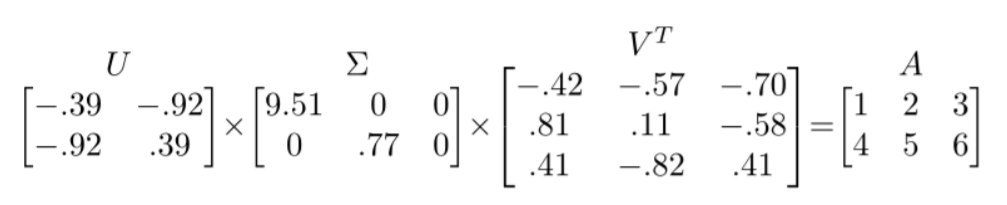
\includegraphics[scale = 0.5]{usigv_example}
\item For many readers, it may be sufficient to extract SVD values by writing: [U, S, V] = numpy.linalg.svd(A). However, the underpinnings of how SVD is computed is useful for later topics. Computers typically compute SVD by taking the following steps:
	\begin{itemize}
    	\item Compute the eigenvectors of $AA^{T}$. These vectors are the columns of U. Square root of the eigenvalues are the singular values (entries of $\Sigma$)
        \item Compute the eigenvectors of $A^{T}A$. These vectors are columns of V (or rows of $V^{T}$)
    \end{itemize}
\item Since SVD relies on eigenvector computation, which are typically fast, SVD can be performed quite quickly; even for large matrices.
\item A more detailed, geometric explanation of SVD may be found here\cite{ams}.
\end{itemize}

\subsection{Applications of Singular Value Decomposition}
\begin{itemize}
\item One the most utilized applications of SVD is the computation of matrix inverses. If an arbitrary matrix A can be decomposed by way of: $A = U\Sigma V^T$, the inverse of A may be defined as: $A^{+} = V^T \Sigma^{-1}U$. Although this inverse is an approximation, it allows one to calculate the inverses of many non-square matrices. MacAusland (2014) discusses the mathematical basis of this inverse, which is named the Moore-Penrose inverse, after its creators\cite{moore-penrose}. Unsurprisingly, a large variety of matrix problems can be solved be utilizing this approach. 
\item Singular Value Decomposition can also be used to compute the Principal Components of a matrix. Principal Components are heavily utilized in various data analysis and machine learning routines, hence SVD is typically a core routine within many programs.
\end{itemize}

\section{Principal Component Analysis}

\subsection{What are Principal Components?}
Continuing with the SVD example we have above, notice that Column 1 of U gets scaled by the first value from $\Sigma$.\\

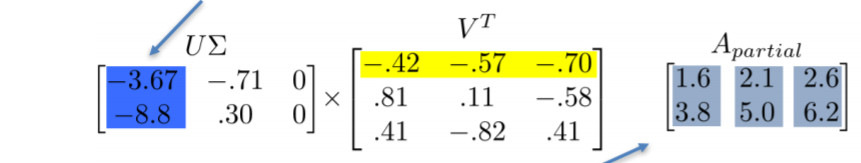
\includegraphics[scale = 0.5]{Usig}

Then, the resulting vector U$\Sigma$ gets scaled by row 1 of $V^T$ to produce a contribution to the columns of A which is denoted $A_{partial}$. Each product of (column i of U)*(value i from $\Sigma$)*(row i of $V^T$) produces a component of the final A.\\

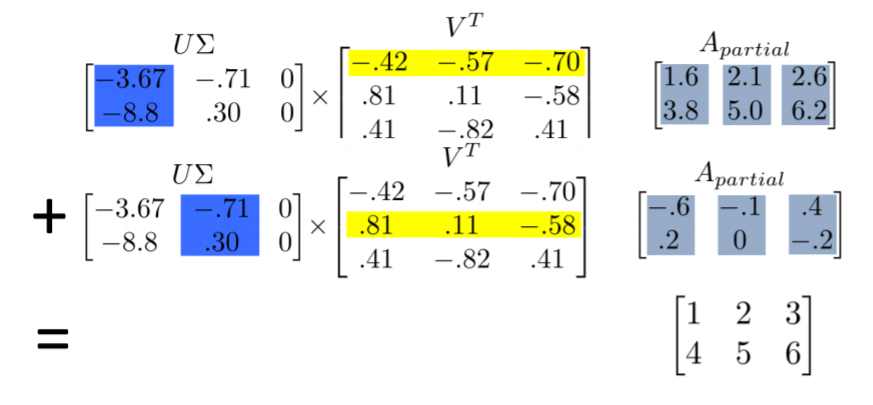
\includegraphics[scale = 0.5]{full_pca}

In this process we are building the the matrix A as a linear combination of the columns of U. As seen above, if we use all columns of U, we rebuild A perfectly. However, in real-world data, \textbf{we can use only the first few columns of U} to get a good approximation of A. This arises due to the properties of $\Sigma$. $\Sigma$ is a diagonal matrix where the largest value is in the top left corner, and the rest of the values on the diagonal decreases as you move to the right. Thus, the first few columns of $U$ contribute the largest weight towards $A$. These first few columns of U are called \textbf{principal components}.\\

However, not all matrices can be easily compressed as in the previous example. One way to evaluate the feasibility is Principal Component Analysis. From a high level standpoint, we want to see if it's possible to remove dimensions that don't contribute much to the final image. We achieve this by analyzing the covariance matrix. Although the value of covariance doesn't matter as much, the sign of covariance does, with positive indicating positive correlation and negative indicating negative correlation. A covariance of zero indicates the two are independent of one another.

\subsection{Performing Principal Component Analysis}
Principal Component Analysis can be performed using the sklearn package:
sklearn.decomposition.PCA. However, it was alluded to earlier that SVD can be used to perform Principal Component Analysis. A non-formal approach is outlined below:

\begin{enumerate}
\item Format your data into a $m * n$ matrix where $m$ denotes the number of samples and $p$ represents the number of features or variables corresponding to a single sample.
\item Center the matrix $X$ by subtracting the mean and dividing by the standard deviation along each column(feature) in $X$
\item Diagonalizing X using SVD yields: $X = U\Sigma V^{T}$
\item Eigenvectors are the principal directions and the projections on these axises are the components. This ultimately means we want to compute $XV$
\item Since V holds eigenvectors and is thus orthonormal, $XV = U\Sigma V^{T}V = US$
\item (5) implies we simply need the columns of $US$, both matrices that are surfaced by SVD
\end{enumerate}

Detailed explanations that elucidate the reasoning behind the above steps are discussed by Moore (1981) and can be found on numerous websites online.

\subsection{Applications of Principal Components}
\begin{itemize}
\item \begin{minipage}[t]{\linewidth}
	PCA has been extensively used in image compression. Much of the 	information captured within an image matrix can be extracted using matrices of lower ranks. This allows large images to be compressed without significant loss of quality. An example of PCA based compression, using only the first 16 principal components, is shown below:\\

  \centering
  
\includegraphics[width=\textwidth]{compare}
  \captionof{figure}{Right: Original Image, Left: Compressed Image}
  \label{fig:sample_figure}

\raggedright
$\,$\\
With just the first 16 principal components, an image that closely resembles the original image can be reconstructed. The relative error as a result of the dimensions used for PCA for the above image is shown below:

  \centering
  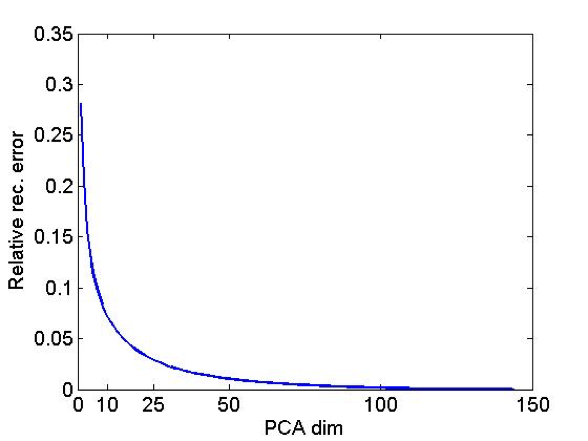
\includegraphics[width=\textwidth]{PCA_dim}
  \captionof{figure}{Relative Error as Function of PCA dimensions}
  \label{fig:sample_figure}
\end{minipage}

\item Web search engines also utilize PCA. There are billions of pages on the Internet that may have a non-trivial relation to a provided search phrase. Companies such as Google, Bing and Yahoo typically narrow the search space by only considering a small subset of this search matrix, which can be extracted using PCA\cite{search-clustering}. This is critical for timely and efficient searches, and it speaks to the power of SVD.
\end{itemize}

In essence, PCA represents data samples as weights on various components - allowing one to essentially represent the difference between samples. This can significantly reduce data redundancy and can make algorithms used in a variety of industries more efficient and insightful!

% References
\small
\bibliographystyle{plain}
\bibliography{bibliography}
\end{document}
